% Геометрические примитивы.
\subsection{Геометрические примитивы, используемые в главе}

\subsubsection{Основные понятия}


Треугольник с вершинами $A$, $B$, $C$, обозначаемый $Tri(A, B, C)$, будем определять как ГМТ $\overline{P}(\beta, \gamma)$ в пространстве, заданное следующим образом:

\begin{equation}\label{eqn:text_1_geo_prim_triangle}
	\left\{
		\begin{aligned}
			& \overline{P}(\beta, \gamma) = \overline{A} + \beta \overline{AB} + \gamma \overline{AC}, \ \beta \in \mathbb{R}, \ \gamma \in \mathbb{R} \\
			& \beta \ge 0 \\
			& \gamma \ge 0 \\
			& \beta + \gamma \le 1
		\end{aligned}
	\right.
\end{equation}

Прямоугольный параллелепипед будем определять как ГМТ $\overline{P} = (x, y, z)$ в пространстве, удовлетворяющих следующей системе неравенств:
\begin{equation}\label{eqn:text_1_geo_prim_parallelepiped}
	\left\{
		\begin{aligned}
			& x_l \le x \le x_h \\
			& y_l \le y \le y_h \\
			& z_l \le z \le z_h
		\end{aligned}
	\right.
\end{equation}

Для такого прямоугольного параллелепипеда будем использовать обозначение $Box([x_l, x_h], [y_l, y_h], [z_l, z_h])$.

\subsubsection{Задача о пересечении треугольника и прямоугольного \\ параллелепипеда в пространстве}\label{sec:text_1_geo_prim_tri_and_parallelepiped_int}

Пусть в пространстве определены треугольник $Tri(A, B, C)$ и прямоугольный параллелепипед $Box([x_l, x_h], [y_l, y_h], [z_l, z_h])$.
Требуется определить, имеют ли они общие точки (см. рис.~\ref{fig:text_1_geo_prim_tri_block_intersect}).

\begin{figure}[ht]
\centering
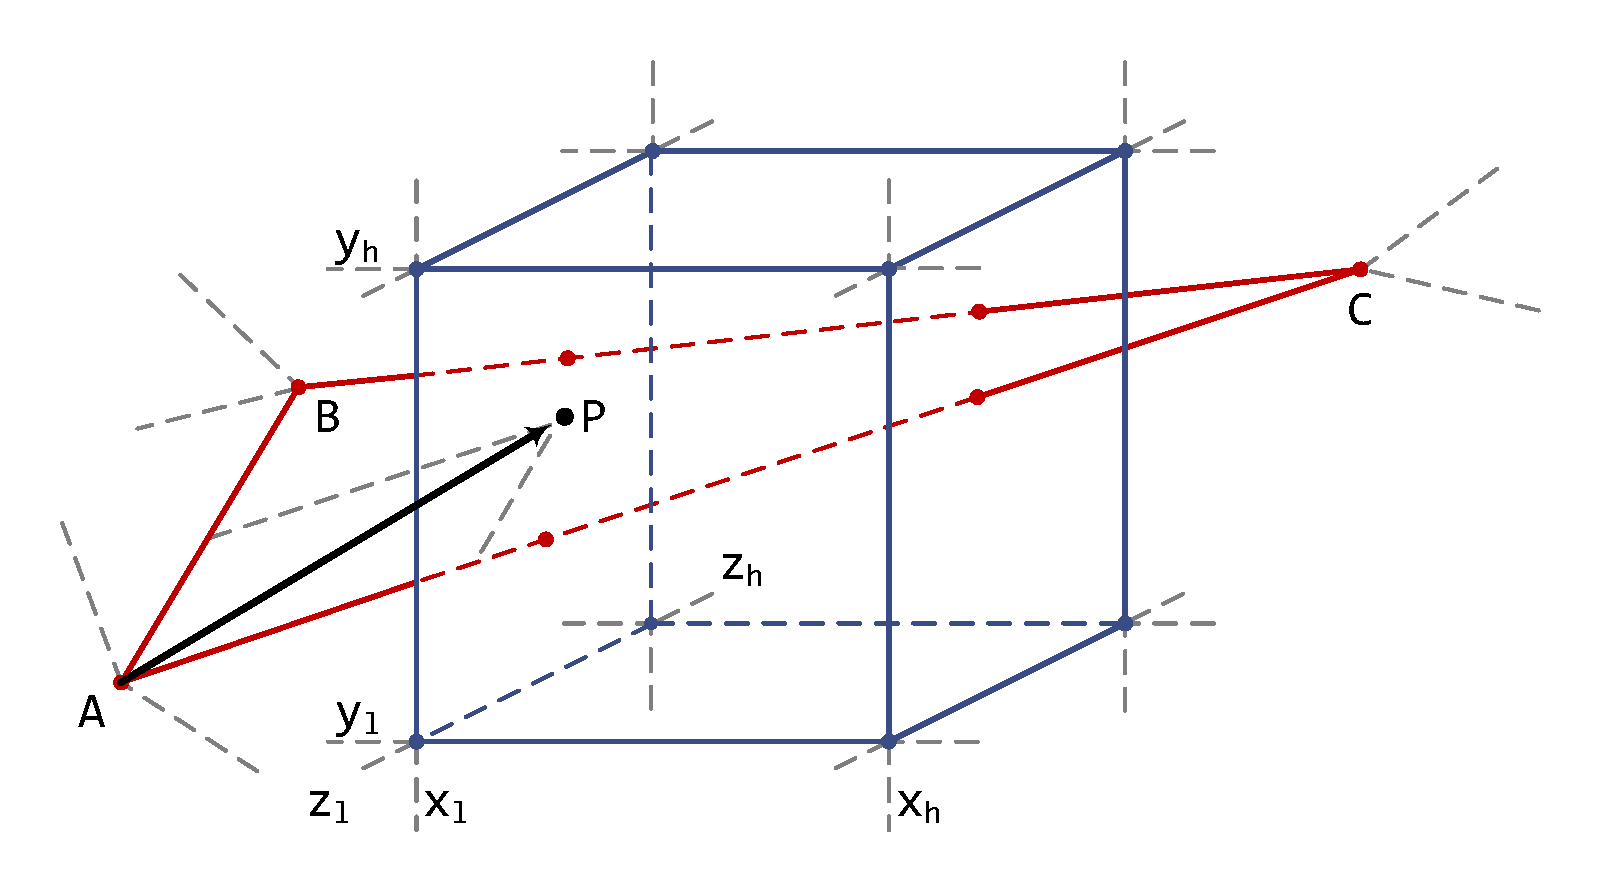
\includegraphics[width=0.7\textwidth]{./pics/text_1_geo_prim/tri_block_intersect.pdf}
\singlespacing
\captionstyle{center}\caption{Пересечение прямоугольного параллелепипеда и треугольника.}
\label{fig:text_1_geo_prim_tri_block_intersect}
\end{figure}

Для решения этой задачи подставим $\overline{P}(\beta, \gamma)$ из \eqref{eqn:text_1_geo_prim_triangle} в систему неравенств \eqref{eqn:text_1_geo_prim_parallelepiped}, получив следующую систему неравенств с двумя переменными $\beta$ и $\gamma$:
\begin{equation}\label{eqn:text_1_geo_prim_1}
	\left\{
		\begin{aligned}
			& x_l \le x_A + \beta (x_B - x_A) + \gamma (x_C - x_A) \le x_h \\
			& y_l \le y_A + \beta (y_B - y_A) + \gamma (y_C - y_A) \le y_h \\
			& z_l \le z_A + \beta (z_B - z_A) + \gamma (z_C - z_A) \le z_h \\
			& \beta \ge 0 \\
			& \gamma \ge 0 \\
			& \beta + \gamma \le 1
		\end{aligned}
	\right.
\end{equation}

Cистема \eqref{eqn:text_1_geo_prim_1} может быть решена методом свертывания конечных систем линейных неравенств \cite{Chernikov1963}\label{term:method_svert_sys_neravenstv}.
Для применения метода свертывания систем линейных неравенств неравенства системы \eqref{eqn:text_1_geo_prim_1} необходимо привести к виду $k_{\beta}\beta + k_{\gamma}\gamma + k \le 0$, после чего получим следующую систему неравенств:
\begin{equation}\label{eqn:text_1_geo_prim_2}
	\left\{
		\begin{aligned}
			& (x_B - x_A) \beta + (x_C - x_A) \gamma + (x_A - x_h) \le 0 \\
			& (x_A - x_B) \beta + (x_A - x_C) \gamma + (x_l - x_A) \le 0 \\
			& (y_B - y_A) \beta + (y_C - y_A) \gamma + (y_A - y_h) \le 0 \\
			& (y_A - y_B) \beta + (y_A - y_C) \gamma + (y_l - y_A) \le 0 \\
			& (z_B - z_A) \beta + (z_C - z_A) \gamma + (z_A - z_h) \le 0 \\
			& (z_A - z_B) \beta + (z_A - z_C) \gamma + (z_l - z_A) \le 0 \\
			& -1 \cdot \beta + 0 \cdot \gamma \le 0 \\
			& 0 \cdot \beta + (-1) \cdot \gamma \le 0 \\
			& \beta + \gamma + (-1) \le 0
		\end{aligned}
	\right.
\end{equation}

Cистема неравенств \eqref{eqn:text_1_geo_prim_2} является системой с двумя переменными ($\beta$ и $\gamma$), поэтому после выполнения одного шага свертывания (деформации)\label{term:deform_sys_lin_neravenstv} она превратится в систему неравенств с одной переменной.
Деформация системы для исключения из нее переменной $\beta$ выполняется следующим образом.
Составляется новая система неравенств, в которую войдут все неравенства системы \eqref{eqn:text_1_geo_prim_2} вида $k_{\gamma} \gamma + k \le 0$, а каждая пара неравенств
\begin{equation}
	\begin{aligned}
		k_{\beta}^1 \beta + k_{\gamma}^1 \gamma + k^1 \le 0 \\
		k_{\beta}^2 \beta + k_{\gamma}^2 \gamma + k^2 \le 0
	\end{aligned}
\end{equation}

в которой коэффициенты при $\beta$ удовлетворяют неравенствам $k_{\beta}^1 < 0$ и $k_{\beta}^2 > 0$, войдет в деформированную систему неравенств в виде
\begin{equation}
	(k_{\gamma}^1 k_{\beta}^2 - k_{\gamma}^2 k_{\beta}^1) \gamma + (k^1 k_{\beta}^2 - k^2 k_{\beta}^1) \le 0. 
\end{equation}

Так как система \eqref{eqn:text_1_geo_prim_2} содержит 9 неравенств, из которых хотя бы в одном коэффициент при $\beta$ нулевой, не более чем в четырех –- положительный, и не более чем в четырех -- отрицательный, то в результате выполнения деформации получим систему, состоящую не более чем из 17 неравенств.
Если деформированная система неравенств с одной переменной имеет решение, то исходные треугольник и прямоугольный параллелепипед имеют общие точки.

\subsubsection{Задача поиска точек пересечения двух треугольников \\ в пространстве}\label{sec:text_1_geo_prim_tri_tri}

Сначала рассмотрим задачу пересечения треугольника и отрезка в пространстве.
Пусть в пространстве задан треугольник $Tri(A, B, C)$ и отрезок $Segm(P, Q)$.
Для поиска точек пересечения этого треугольника и отрезка требуется найти решение следующей системы уравнений
\begin{equation}\label{eqn:text_1_geo_prim_tri_segm_int}
	\left\{
		\begin{aligned}
			& x_A + (x_B - x_A) \beta + (x_C - x_A) \gamma = x_P + (x_Q - x_P) \alpha \\
			& y_A + (y_B - y_A) \beta + (y_C - y_A) \gamma = y_P + (y_Q - y_P) \alpha \\
			& z_A + (z_B - z_A) \beta + (z_C - z_A) \gamma = z_P + (z_Q - z_P) \alpha
		\end{aligned}
	\right.
\end{equation}

при ограничениях $0 \le \alpha \le 1$, $\beta \ge 0$, $\gamma \ge 0$, $\beta + \gamma \le 1$.

Система уравнений \eqref{eqn:text_1_geo_prim_tri_segm_int} может не иметь решений, может иметь ровно одно решение (если прямая $Line(P, \overline{PQ})$ пересекает плоскость треугольника) либо имеет бесконечное количество решений (если прямая $Line(P, \overline{PQ})$ лежит в плоскости треугольника).

\begin{figure}[ht]
\centering
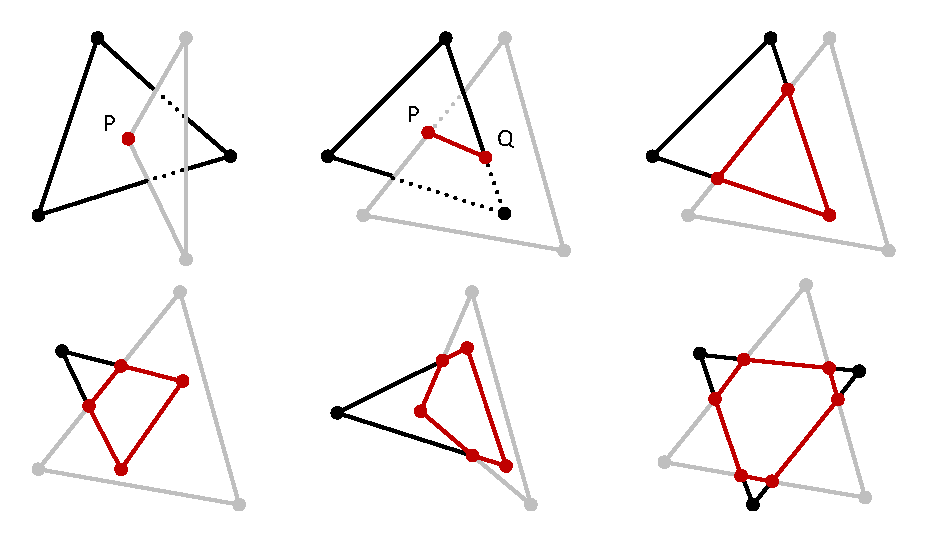
\includegraphics[width=0.7\textwidth]{./pics/text_1_geo_prim/tri_tri.pdf}
\singlespacing
\captionstyle{center}\caption{Пересечение двух треугольников в пространстве.}
\label{fig:text_1_geo_prim_tri_tri}
\end{figure}

Пусть теперь в пространстве заданы два треугольника.
Так как треугольник является выпуклой фигурой, то пересечение двух треугольников либо пусто, либо также является выпуклой фигурой (это может быть плоская фигура с количеством вершин от 1 до 6, см. рис.~\ref{fig:text_1_geo_prim_tri_tri}).

Вершины области пересечения двух треугольников это точки пересечения трех сторон первого треугольника со вторым треугольником и наоборот.
То есть для поиска вершин области пересечения двух треугольников нужно решить 6 задач пересечения треугольника с отрезком в пространстве.
